\section{Function Approximation}


\subsection{Problem 5.9}


\begin{figure}[!ht]
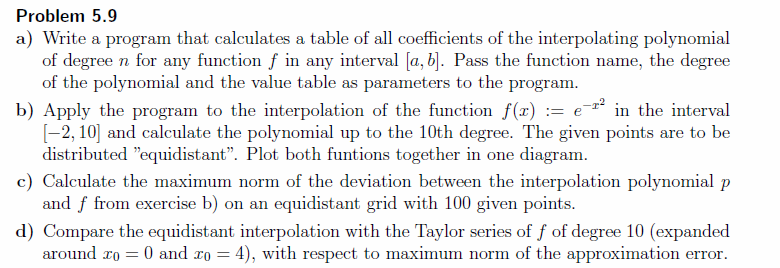
\includegraphics[width=1\textwidth]{chapters/images/desc-5-9}
\end{figure}


\subsubsection{a)}

To calculate the coefficients, [...]

[numpy to solve lin eq]

\begin{lstlisting}[caption=Problem 5.9 a)]
def getCoefficients(fx, degree, a, b):
	xses = [];
	yses = [];
	
	step = (b - a) / float(degree - 1);
	
	for i in range(degree):
		x = a + i * step;
		xses.append(x);
		yses.append(fx(x));
	
	matA = [];
	
	for xVal in xses:
		row = [];
		for i in range(degree):
			row.append(pow(xVal, i));
		
		matA.append(row);
	
	matrixArr = np.array(matA);
	vectorArr = np.array(yses);
	
	linSolutions = np.linalg.solve(matrixArr, vectorArr);
	
	return linSolutions;
\end{lstlisting}

This function will be used in the following subtasks.


\subsubsection{b)}

To use the coefficients as a function, a python function to [return a value is required].

\begin{lstlisting}[caption=Function which uses the calculated coefficients]
def polynomialF(coefficients, x):
	sum = 0.0;
	
	for i in range(len(coefficients)):
		sum += coefficients[i] * pow(x, i);
	
	return sum;
\end{lstlisting}

[now plot them]

\begin{lstlisting}[caption=todo]
def myF(x):
	return pow(math.e, -pow(x, 2));

coefficients = getCoefficients(myF, 10, -2, 10);

xses = [];
realYses = [];
approxYses = [];

for i in range(100):
	x = -2 + i * (12 / 100.0);
	
	xses.append(x);
	realYses.append(myF(x));
	approxYses.append(polynomialF(coefficients, x));

plt.plot(xses, realYses);
plt.plot(xses, approxYses);
plt.xlabel("x");
plt.ylabel("y");
plt.show();
\end{lstlisting}

[the resulting plot looks like the following]

%\begin{figure}[h!]
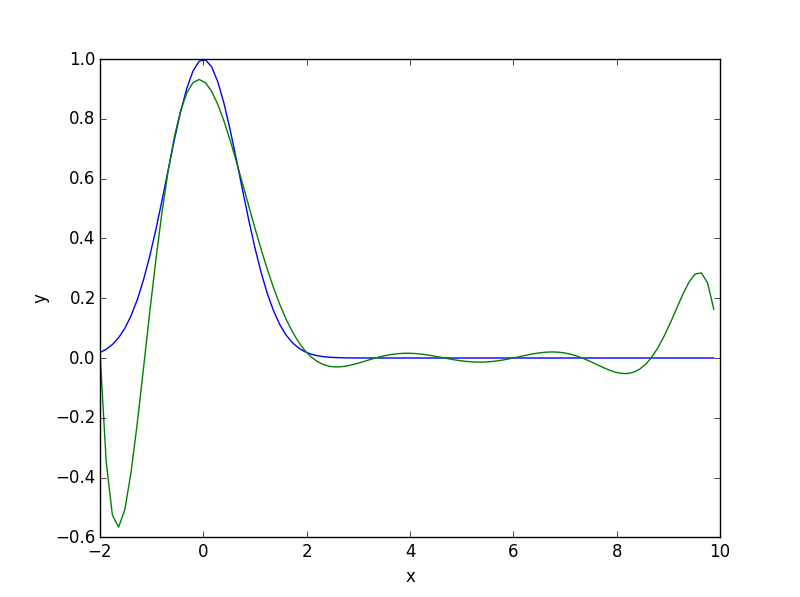
\includegraphics[width=1\textwidth]{chapters/images/figure-5-9-b}
%\caption{Plot of the }
%\end{figure}

\begin{figure}[h!]
%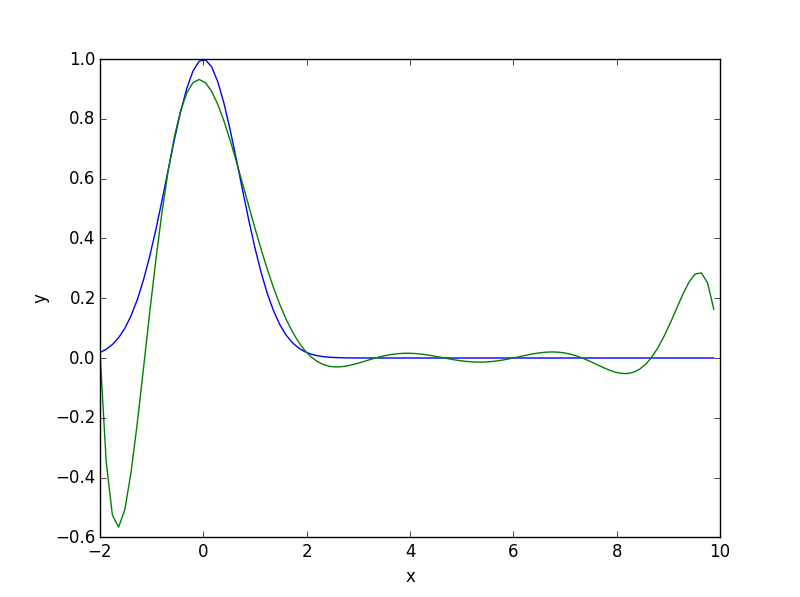
\includegraphics[width=1\textwidth]{chapters/images/figure-5-9-b}
\caption{Plot of both functions}
\end{figure}

[blue - real, green - approx]
[close to origin in the positive part pretty equal]


\subsubsection{c)}

\begin{lstlisting}[caption=Problem 5.9 c)]
maxApproxDev = -1;

for i in range(100):
	realY = realYses[i];
	approxY = approxYses[i];
	
	maxApproxDev = max(maxApproxDev, abs(realY - approxY));

print("maximum deviation: " + str(maxApproxDev));
\end{lstlisting}


The results of the calculation of the maximum deviation are:

\begin{lstlisting}[caption=Result of 5.9 c), keywordstyle=\color{black}]
maximum deviation: 0.634025332357
\end{lstlisting}


\subsubsection{d)}

[First Taylor Series]

[Calc Yses for Plot]

\begin{lstlisting}[caption=todo]
def taylorFuncAt0(x):
	sum = 1;
	sum -= pow(x, 2);
	sum += pow(x, 4) / 2.0;
	sum -= pow(x, 6) / 6.0;
	sum += pow(x, 8) / 24.0;
	sum -= pow(x, 10) / 120.0;
	sum += pow(x, 12) / 720.0;
	sum -= pow(x, 14) / 5040.0;
	sum += pow(x, 16) / 40320.0;
	
	return sum;

def taylorFuncAt4(x):
	ep16 = float(pow(math.e, 16));
	xm4 = x - 4;
	
	sum = 1 / ep16;
	sum -= 8 * xm4 / ep16;
	sum += 31 * pow(xm4, 2) / ep16;
	sum -= 232 * pow(xm4, 3) / (3 * ep16);
	sum += 835 * pow(xm4, 4) / (6 * ep16);
	sum -= 2876 * pow(xm4, 5) / (15 * ep16);
	sum += 18833 * pow(xm4, 6) / (90 * ep16);
	sum -= 58076 * pow(xm4, 7) / (315 * ep16);
	sum += 332777 * pow(xm4, 8) / (2520 * ep16);
	sum -= 43325 * pow(xm4, 9) / (567 * ep16);
	sum += 3937007 * pow(xm4, 10) / (113400 * ep16);
	
	return sum;

taylor0Yses = [];
taylor4Yses = [];

for i in range(100):
	x = -2 + i * (12 / 100.0);
	
	taylor0Yses.append(taylorFuncAt0(x));
	taylor4Yses.append(taylorFuncAt4(x));
\end{lstlisting}

[Then calculate deviation]

\begin{lstlisting}[caption=todo]

maxTaylor0Dev = -1;
maxTaylor4Dev = -1;

for i in range(100):
	realY = realYses[i];
	taylor0Y = taylor0Yses[i];
	taylor4Y = taylor4Yses[i];
	
	maxTaylor0Dev = max(maxTaylor0Dev, abs(realY - taylor0Y));
	maxTaylor4Dev = max(maxTaylor4Dev, abs(realY - taylor4Y));

print("maximum deviation of taylor series with c = 0: " + str(maxTaylor0Dev));
print("maximum deviation of taylor series with c = 4: " + str(maxTaylor4Dev));
\end{lstlisting}

[the results are]

\begin{lstlisting}[caption=Result of 1.1 a), keywordstyle=\color{black}]
maximum deviation of taylor series with c = 0: 1.88827128486e+11
maximum deviation of taylor series with c = 4: 354.936464804
\end{lstlisting}

[taylor at $c = 0$ with much bigger deviation]

[because $c = 4$ is the center of interval]


\subsection{Problem 5.10}


\begin{figure}[!ht]
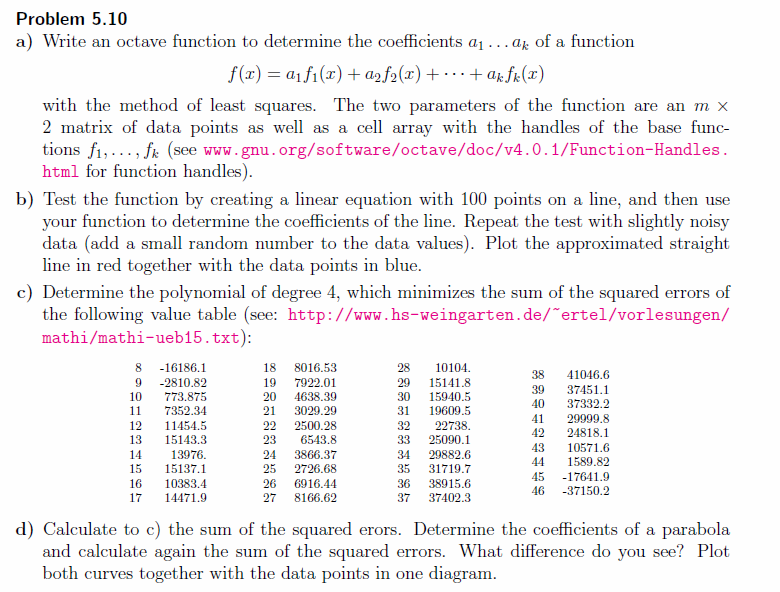
\includegraphics[width=1\textwidth]{chapters/images/desc-5-10}
\end{figure}


\subsubsection{a)}

[get coefficients with method of least squares]

[again lin eq can be solved with numpy]

\begin{lstlisting}[caption=Problem 5.10 a)]
def getCoefficients(baseFunctions, dataPoints):
	l = len(baseFunctions);
	
	matA = [];
	
	for i in range(l):
		matrixRow = [];
		for j in range(l):
			elemSum = 0;
		
			for dp in dataPoints:
				x = dp[0];
				elemSum += baseFunctions[i](x) * baseFunctions[j](x);
			
			matrixRow.append(elemSum);
		
		matA.append(matrixRow);
	
	vecB = [];
	
	for i in range(l):
		elemSum = 0;
	
		for dp in dataPoints:
			elemSum += dp[1] * baseFunctions[i](dp[0]);
		
		vecB.append(elemSum);
	
	matrixArr = np.array(matA);
	vectorArr = np.array(vecB);
	
	linSolutions = np.linalg.solve(matrixArr, vectorArr);
	
	return linSolutions;
\end{lstlisting}


\subsubsection{b)}

[with the function from a), simple to make the lin eq with two base functions.]

[afterwards, calculate enough y values and plot them]

\begin{lstlisting}[caption=todo]
def myF1(x): return x;
def myF0(x): return 1;

baseFns = [];

baseFns.append(myF1);
baseFns.append(myF0);

linPoints = [];
rndPoints = [];
xses = [];
yses = [];
rndYses = [];

for i in range(100):
	x = i / 10.0;
	y = x * 0.64 + 2.3;
	
	xses.append(x);
	yses.append(y);

	rnd = random.random() - 0.5;
	rndY = y + rnd * 0.6;
	rndYses.append(rndY);
	
	linPoints.append([x, y]);
	rndPoints.append([x, rndY]);

print("coefficients:");
print(getCoefficients(baseFns, linPoints));

print("approximated coefficients:");
print(getCoefficients(baseFns, rndPoints));

plt.plot(xses, yses);
plt.plot(xses, rndYses, "ro");
plt.xlabel("x");
plt.ylabel("y");
plt.show();
\end{lstlisting}


[The result of the exact coefficients and the approximation with random points are]

\begin{lstlisting}[caption=Result of 1.1 a), keywordstyle=\color{black}]
coefficients:
[ 0.64   0.23 ]

approximated coefficients:
[ 0.63139257   2.33442881 ]
\end{lstlisting}

[the approximated coefficients are very close.]

[the plot of the exact linear equation and the random points looks like this:]

\begin{figure}[!ht]
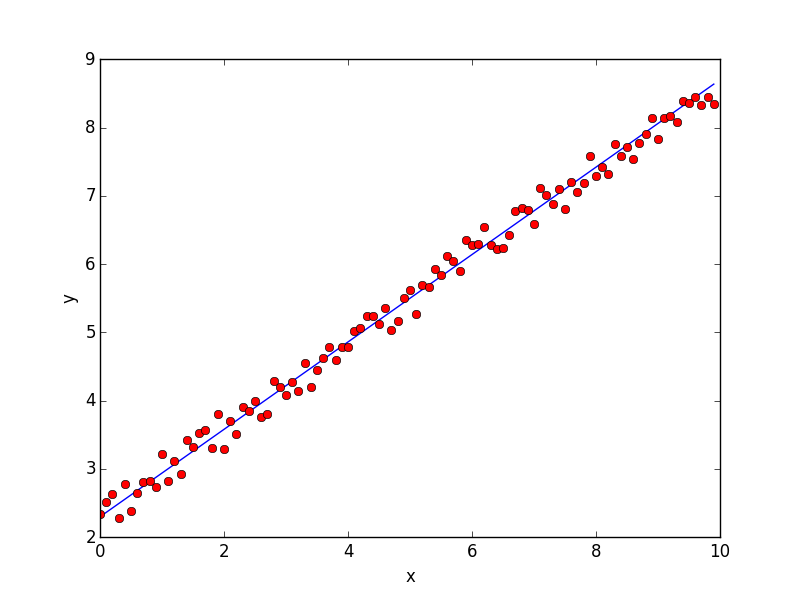
\includegraphics[width=1\textwidth]{chapters/images/figure-5-10-b}
\caption{todo}
\end{figure}


\subsubsection{c)}

[also with the function, poly degree 4 and 2 which is needed for subtask d)]

\begin{lstlisting}[caption=todo]
def myF4(x): return pow(x, 4);
def myF3(x): return pow(x, 3);
def myF2(x): return pow(x, 2);
def myF1(x): return x;
def myF0(x): return 1;

def polynomialF(coefficients, x):
	sum = 0.0;
	
	nc = len(coefficients);
	
	for i in range(nc):
		sum += coefficients[i] * pow(x, nc - i - 1);
	
	return sum;

txtBaseFns4 = [];
txtBaseFns2 = [];

txtBaseFns4.append(myF4);
txtBaseFns4.append(myF3);
txtBaseFns4.append(myF2);
txtBaseFns4.append(myF1);
txtBaseFns4.append(myF0);

txtBaseFns2.append(myF2);
txtBaseFns2.append(myF1);
txtBaseFns2.append(myF0);

txtPoints = [];

txtPoints.append([8, -16186.1]);
txtPoints.append([9, -2810.82]);
# [...] (I left out the other values in the paper to save space)
txtPoints.append([45, -17641.9]);
txtPoints.append([46, -37150.2]);

txtCoefficients4 = getCoefficients(txtBaseFns4, txtPoints);
txtCoefficients2 = getCoefficients(txtBaseFns2, txtPoints);

txtPointsXses = [];
txtPointsYses = [];

error4 = 0;
error2 = 0;

for i in range(len(txtPoints)):
	txtPoint = txtPoints[i];
	
	txtPointsXses.append(txtPoint[0]);
	txtPointsYses.append(txtPoint[1]);
	
	y4 = polynomialF(txtCoefficients4, i + 8);
	y2 = polynomialF(txtCoefficients2, i + 8);
	
	error4 += pow(y4 - txtPoint[1], 2);
	error2 += pow(y2 - txtPoint[1], 2);


print("error of degree 4 polynomial: " + str(error4));
print("error of degree 2 polynomial: " + str(error2));

txtFXses = [];
txtF4Yses = [];
txtF2Yses = [];

for i in range(152):
	x = 8 + i * 0.25;
	
	txtFXses.append(x);
	
	y4 = polynomialF(txtCoefficients4, x);
	y2 = polynomialF(txtCoefficients2, x);
	
	txtF4Yses.append(y4);
	txtF2Yses.append(y2);


plt.plot(txtFXses, txtF4Yses);
plt.plot(txtFXses, txtF2Yses);
plt.plot(txtPointsXses, txtPointsYses, "ro");
plt.xlabel("x");
plt.ylabel("y");
plt.show();
\end{lstlisting}


results:

\begin{lstlisting}[caption=Result of 1.1 a), keywordstyle=\color{black}]
R
\end{lstlisting}

X



\subsubsection{d)}

[use the functions from c) 

\begin{lstlisting}[caption=todo]

siehe c) - aufdroeseln

\end{lstlisting}


results:

\begin{lstlisting}[caption=Result of 1.1 a), keywordstyle=\color{black}]
error of degree 4 polynomial: 101457690.277
error of degree 2 polynomial: 7711489909.2
\end{lstlisting}

[error of degree 4 over 70 times smaller] [makes sense]

[the plot looks like this]

\begin{figure}[!ht]
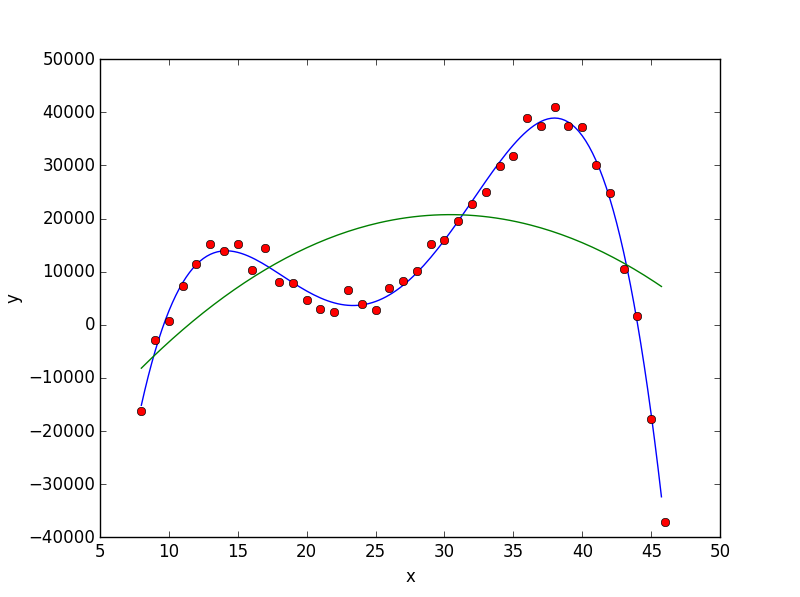
\includegraphics[width=1\textwidth]{chapters/images/figure-5-10-d}
\caption{todo}
\end{figure}

[perfectly illustrates the closeness and farawayness of each function]


\subsection{Problem 5.11}


\begin{figure}[!ht]
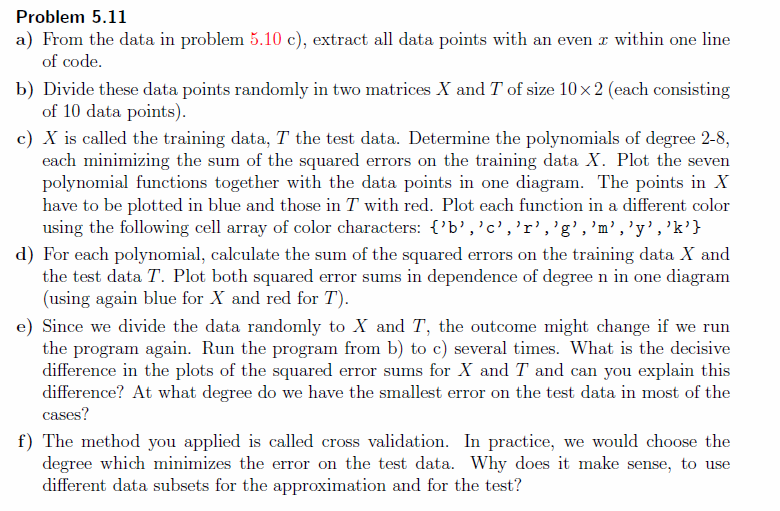
\includegraphics[width=1\textwidth]{chapters/images/desc-5-11}
\end{figure}

The methods $getCoefficients$ and $polynomialF$ as well as the $txtPoints$ from problem 5.10 will be used in this exercise as well.


\subsubsection{a)}

\begin{lstlisting}[caption=todo]
evenPoints = [];

for txtPoint in txtPoints:
	if txtPoint[0] % 2 == 0:
		evenPoints.append(txtPoint);
\end{lstlisting}


\subsubsection{b)}

\begin{lstlisting}[caption=todo]
matrixX = [];
matrixT = [];

for evenPoint in evenPoints:
	rnd = random.random();
	
	if len(matrixT) >= 10 or (rnd < 0.5 and len(matrixX) < 10):
		matrixX.append(evenPoint);
	else:
		matrixT.append(evenPoint);
\end{lstlisting}


\subsubsection{c)}

[To get the polynomials up to degree 8, first the base functions have to be defined:]

\begin{lstlisting}[caption=todo]
def myF8(x): return pow(x, 8);
def myF7(x): return pow(x, 7);
def myF6(x): return pow(x, 6);
def myF5(x): return pow(x, 5);
def myF4(x): return pow(x, 4);
def myF3(x): return pow(x, 3);
def myF2(x): return pow(x, 2);
def myF1(x): return x;
def myF0(x): return 1;

def getBaseFunctionList(degree):
	baseFunctions = [];
	
	if degree >= 8: baseFunctions.append(myF8);
	if degree >= 7: baseFunctions.append(myF7);
	if degree >= 6: baseFunctions.append(myF6);
	if degree >= 5: baseFunctions.append(myF5);
	if degree >= 4: baseFunctions.append(myF4);
	if degree >= 3: baseFunctions.append(myF3);
	if degree >= 2: baseFunctions.append(myF2);
	
	baseFunctions.append(myF1);
	baseFunctions.append(myF0);
	
	return baseFunctions;
\end{lstlisting}

[using these base functions the coefficients can be calculated with the $getCoefficients$ function. Afterwards, the y values of those functions can be collected with the $polynomialF$ function to plot them].

\begin{lstlisting}[caption=todo]
xses = [];
allYses = [];

for i in range(152):
	xses.append(8 + i * 0.25);

for i in range(7):
	degree = i + 2;
	
	baseFunctionList = getBaseFunctionList(degree);
	
	coefficients = getCoefficients(baseFunctionList, matrixX);
	
	yses = [];
	
	for x in xses:
		y = polynomialF(coefficients, x);
		yses.append(y);
	
	allYses.append(yses);

xXses = [];
xYses = [];
tXses = [];
tYses = [];

for i in range(10):
	xXses.append(matrixX[i][0]);
	xYses.append(matrixX[i][1]);
	tXses.append(matrixT[i][0]);
	tYses.append(matrixT[i][1]);

colors = ["b", "c", "r", "g", "m", "y", "k"];

plt.plot(xXses, xYses, "bo");
plt.plot(tXses, tYses, "ro");

for i in range(len(allYses)):
	plt.plot(xses, allYses[i], colors[i]);

plt.xlabel("x");
plt.ylabel("y");
plt.show();
\end{lstlisting}

[the resulting graph looks like this.]

\begin{figure}[!ht]
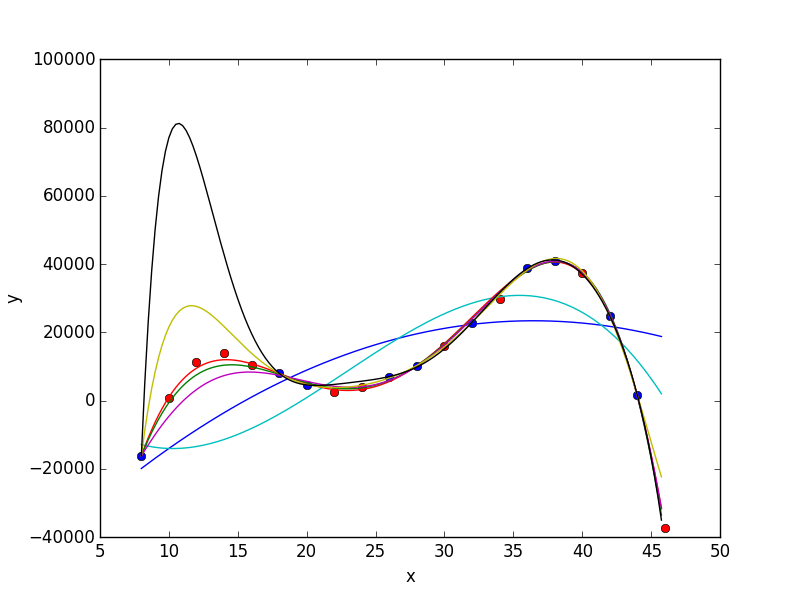
\includegraphics[width=1\textwidth]{chapters/images/figure-5-11-c}
\caption{todo}
\end{figure}


\subsubsection{d)}

[to calculate the error, square of distance between data point]

\begin{lstlisting}[caption=todo]
def getError(coefficients, mat):
	errorSum = 0;
	
	for elem in mat:
		fY = polynomialF(coefficients, elem[0]);
		
		errorSum += pow(fY - elem[1], 2);
	
	return errorSum;

def getErrors(degree, matX, matT):
	baseFunctionList = getBaseFunctionList(degree);
	
	coefficients = getCoefficients(baseFunctionList, matX);
	
	errorSumX = getError(coefficients, matX);
	errorSumT = getError(coefficients, matT);
	
	return [errorSumX, errorSumT];

degrees = [];
errorsX = [];
errorsT = [];

for i in range(7):
	degree = i + 2;
	degrees.append(degree);
	
	errors = getErrors(degree, matrixX, matrixT);
	
	errorsX.append(errors[0]);
	errorsT.append(errors[1]);

plt.plot(degrees, errorsX, "b");
plt.plot(degrees, errorsT, "r");

plt.xlabel("degree");
plt.ylabel("error");
plt.show();
\end{lstlisting}

[the result looks the following:]

\begin{figure}[!ht]
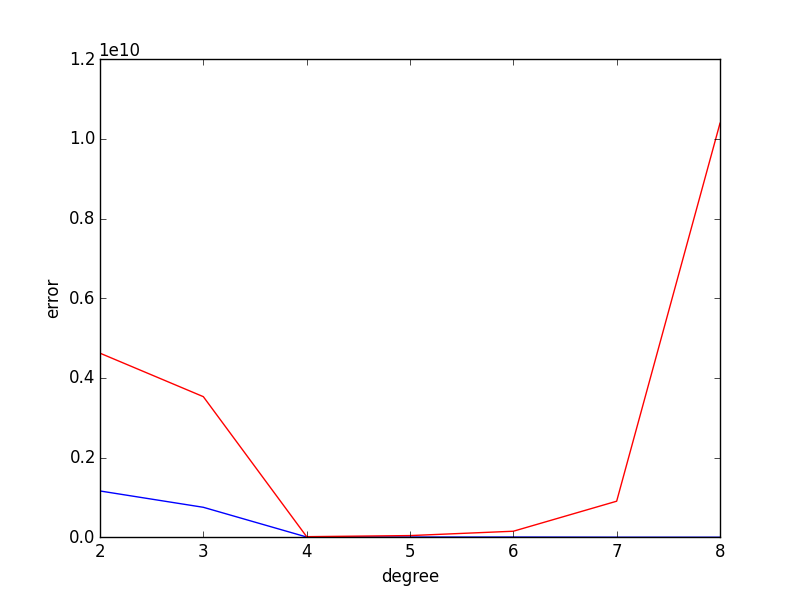
\includegraphics[width=1\textwidth]{chapters/images/figure-5-11-d}
\caption{todo}
\end{figure}


\subsubsection{e)}

[with a higher degree, the deviation from training data is pretty small]. [obv since they are used for the small function]

[on the test data however the error first drops but then increases]

The deviation to the original approximated function (where all data points were used) minimizes the more evenly the points of X and T are distributed. The reason for that is that when there's a large interval of test points only, the approximated function has no bounds at all in that interval and can deviate as much as it needs to, without increasing the error.
The results seems to be the the best with polynomials of degree 4 and 5.

[a reason could be that functions of higher degrees tend to spike more, and they are more free with \enquote{loose} test data points]

\subsubsection{f)}

It makes sense because the approximated function is supposed to be close to all data values, and even the points \enquote{in between} which are not part of both the training and test data.